\documentclass{beamer}

\usepackage{geometry}
\usepackage{graphicx}
%\usepackage{wrapfig}
\usepackage{amsmath}

%\useoutertheme{infolines}
\usetheme{Boadilla}
\usecolortheme{seahorse}
\setbeamertemplate{navigation symbols}{}
\title{Bit Operations}
\newcommand{\shorttitle}{64 Bit Intel Assembly Language}
\newcommand{\shortauthor}{\copyright 2011 Ray Seyfarth}
\author{Ray Seyfarth}
\begin{document}


\usefoottemplate{\vbox{
\tinycolouredline{structure!55}%
 {\color{white}{\textbf{\shorttitle}\hfill\textbf{\shortauthor}}}%
}}

\begin{frame}
    \titlepage
\end{frame}

\begin{frame}
\frametitle{Outline}
\tableofcontents
\end{frame}

\section{Introduction to bits}

\begin{frame}
    \frametitle{Bit usage}
    \begin{itemize}
        \item A bit can mean one of a pair of characteristics
        \item True or false
        \item Male or female
        \item Bit fields can represent larger classes
        \item There are 64 squares on a chess board, 6 bits could
              specify a position
        \item The exponent field of a float is bits 30-24 of a double 
              word
        \item We could use a 4 bit field to store a color from black,
              red, green, blue, yellow, cyan, purple and white
        \item Should you store numbers from 0-15 in 4 bits or in a
              byte?
    \end{itemize}
\end{frame}

\begin{frame}
    \frametitle{Bit operations}
    \begin{itemize}
        \item Individual bits have values 0 and 1
        \item There are instructions to perform bit operations
        \item Using 1 as true and 0 as false
        \begin{itemize}
            \item 1 and 1 = 1, or in C, {\tt 1 \&\& 1 = 1}
            \item 1 and 0 = 0, or in C, {\tt 1 \&\& 0 = 0}
            \item 1 or 0 = 1, or in C, {\tt 1 || 0 = 1}
        \end{itemize}
        \item We are interested in operations on more bits
        \begin{itemize}
            \item {\tt 10101000b \& 11110000b = 10100000b}
            \item {\tt 10101000b | 00001010b = 10101010b}
        \end{itemize}
        \item These are called ``bit-wise'' operations
        \item We will not use bit operations on single bits, though we
              will test individual bits
    \end{itemize}
\end{frame}

\section{Not}

\begin{frame}[fragile]
    \frametitle{Not operation}
    \begin{itemize}
        \item C uses {\tt !} for a logical not
        \item C uses {\tt \~{}} for a bit-wise not
    \end{itemize}
\begin{verbatim}
    !0 == 1
    !1 == 0
    ~0 == 1
    ~1 == 0
    ~10101010b == 01010101b
    ~0xff00 == 0x00ff
    !1000000 == 0
\end{verbatim}   
\end{frame}

\begin{frame}[fragile]
    \frametitle{Not instruction}
    \begin{itemize}
        \item The {\tt not} instruction flips all the bits of a number
              - one's complement
        \item {\tt not} leaves the flags alone
        \item There is only a single operand which is source and destination
        \item For memory operands you must include a size prefix
        \item The sizes are {\tt byte}, {\tt word}, {\tt dword} and {\tt qword}
        \item The C operator is 
    \end{itemize}
    \begin{verbatim}
        not     rax       ; invert all bits of rax
        not     dword [x] ; invert double word at x
        not     byte [x]  ; invert a byte at x
    \end{verbatim}
\end{frame}

\section{And}

\begin{frame}[fragile]
    \frametitle{And operation}
\begin{center}
\begin{tabular}{c|cc}
{\tt \&} & 0 & 1 \\
\hline
0       & 0 & 0 \\
1       & 0 & 1 \\
\end{tabular}
\end{center}
    \begin{itemize}
        \item C uses {\tt \&} for a logical and
        \item C uses {\tt \&\&} for a bit-wise and
    \end{itemize}
\small
\begin{verbatim}
    11001100b & 00001111b == 00001100b
    11001100b & 11110000b == 11000000b
    0xabcdefab & 0xff == 0xab
    0x0123456789abcdef & 0xff00ff00ff00ff00 == 0x010045008900cd00
\end{verbatim}
\begin{itemize}
    \item Bit-wise and is a bit selector
\end{itemize}

\end{frame}

\begin{frame}[fragile]
    \frametitle{And instruction}
    \begin{itemize}
        \item The {\tt and} instruction performs a bit-wise and
        \item It has 2 operands, a destination and a source
        \item The source can be an immediate value, a memory location
              or a register
        \item The destination can be a register or memory
        \item Not both destination and source can be memory
        \item The sign flag and zero flag are set (or cleared)
    \end{itemize}

\begin{verbatim}
    mov     rax, 0x12345678
    mov     rbx, rax
    and     rbx, 0xf         ; rbx has the low nibble 0x8
    mov     rdx, 0           ; prepare to divide
    mov     rcx, 16          ; by 16
    idiv    rcx              ; rax has 0x1234567
    and     rax, 0xf         ; rax has the nibble 0x7
\end{verbatim}
\end{frame}

\section{Or}

\begin{frame}[fragile]
    \frametitle{Or operation}
\begin{center}
\begin{tabular}{c|cc}
{\tt |} & 0 & 1 \\
\hline
0       & 0 & 1 \\
1       & 1 & 1 \\
\end{tabular}
\end{center}
    \begin{itemize}
        \item C uses {\tt |} for a logical and
        \item C uses {\tt ||} for a bit-wise and
    \end{itemize}
\small
\begin{verbatim}
    11001100b | 00001111b == 11001111b
    11001100b | 11110000b == 11111100b
    0xabcdefab | 0xff == 0xabcdefff
    0x0123456789abcdef | 0xff00ff00ff00ff00 == 0xff23ff67ffabffef
\end{verbatim}
    \begin{itemize}
        \item Or is a bit setter
    \end{itemize}
\end{frame}

\begin{frame}[fragile]
    \frametitle{Or instruction}
   \begin{itemize}
        \item The {\tt or} instruction performs a bit-wise or
        \item It has 2 operands, a destination and a source
        \item The source can be an immediate value, a memory location
              or a register
        \item The destination can be a register or memory
        \item Not both destination and source can be memory
        \item The sign flag and zero flag are set (or cleared)
    \end{itemize}
\begin{verbatim}
    mov     rax, 0x1000
    or      rax, 1          ; make the number odd
    or      rax, 0xff00     ; set bits 15-8
\end{verbatim}
\end{frame}

\section{Exclusive or}

\begin{frame}[fragile]
    \frametitle{Exclusive or operation}
\begin{center}
\begin{tabular}{c|cc}
{\tt \^{}} & 0 & 1 \\
\hline
0       & 0 & 1 \\
1       & 1 & 0 \\
\end{tabular}
\end{center}
    \begin{itemize}
        \item C uses {\tt \^{}} for exclusive or
    \end{itemize}
\begin{verbatim}
    00010001b ^ 00000001b == 00010000b
    01010101b ^ 11111111b == 10101010b
    01110111b ^ 00001111b == 01111000b
    0xaaaaaaaa ^ 0xffffffff == 0x55555555
    0x12345678 ^ 0x12345678 == 0x00000000
\end{verbatim}
    \begin{itemize}
        \item Exclusive or is a bit flipper
    \end{itemize}
\end{frame}

\begin{frame}[fragile]
    \frametitle{Exclusive or instruction}
    \begin{itemize}
        \item The {\tt xor} instruction performs a bit-wise exclusive
              or
        \item It has 2 operands, a destination and a source
        \item The source can be an immediate value, a memory location
              or a register
        \item The destination can be a register or memory
        \item Not both destination and source can be memory
        \item The sign flag and zero flag are set (or cleared)
        \item {\tt mov rax, 0} uses 7 bytes
        \item {\tt xor rax, rax} uses 3 bytes
        \item {\tt xor eax, eax} uses 2 bytes
    \end{itemize}
\begin{verbatim}
    mov     rax, 0x1234567812345678
    xor     eax, eax                ; set rax to 0
    mov     rax, 0x1234
    xor     rax, 0xf                ; change to 0x123b
\end{verbatim}
\end{frame}

\section{Shift operations}

\begin{frame}[fragile]
    \frametitle{Shift operations}
    \begin{itemize}
        \item C uses {\tt <<} for shift left and {\tt >>} for shift
              right
        \item Shifting left introduces low order 0 bits
        \item Shifting right propagates the sign bit in C for
              signed integers
        \item Shifting right introduces 0 bits in C for
              unsigned integers
        \item Shifting left is like multiplying by a power of 2
        \item Shifting right is like dividing by a power of 2
    \end{itemize}
\begin{verbatim}
    101010b >> 3 == 10b
    111111b << 2 == 11111100b
    125 << 2 == 500
    0xabcd >> 4 == 0xabc
\end{verbatim}
\end{frame}

\begin{frame}
    \frametitle{Shift instructions}
    \begin{itemize}
        \item Shift left: {\tt shl}
        \item Shift right: {\tt shr}
        \item Shift arithmetic left: {\tt sal}
        \item Shift arithmetic right: {\tt sar}
        \item {\tt shl} and {\tt sal} are the same
        \item {\tt shr} introduces 0 bits on the top end
        \item {\tt sar} propagates the sign bit
        \item There are 2 operands
        \begin{itemize}
            \item A destination register or memory
            \item In immediate number of bits to shift or {\tt cl} 
        \end{itemize}
        \item The sign and zero flags are set (or cleared)
        \item The carry flag is set to the last bit shifted out
    \end{itemize}
\end{frame}

\begin{frame}
    \frametitle{Extracting a bit field}
    \begin{itemize}
        \item There are at least 2 ways to extract a bit field
        \item Shift right followed by an and
        \begin{itemize}
            \item To extract bits $m-k$ with $m \ge k$, shift right $k$ bits
            \item And this value with a mask of $m-k+1$ bits all set to 1
        \end{itemize}
        \item Shift left and then right
        \begin{itemize}
            \item Shift left until bit $m$ is the highest bit
            \item With 64 bit registers, shift left $63-m$ bits
            \item Shift right to get original bit $k$ in position 0
            \item With 64 bit registers, shift right $63-(m-k)$ bits
        \end{itemize}
    \end{itemize}
\end{frame}

\begin{frame}
    \frametitle{Extracting a bit field with shift/and}
    \begin{center}
        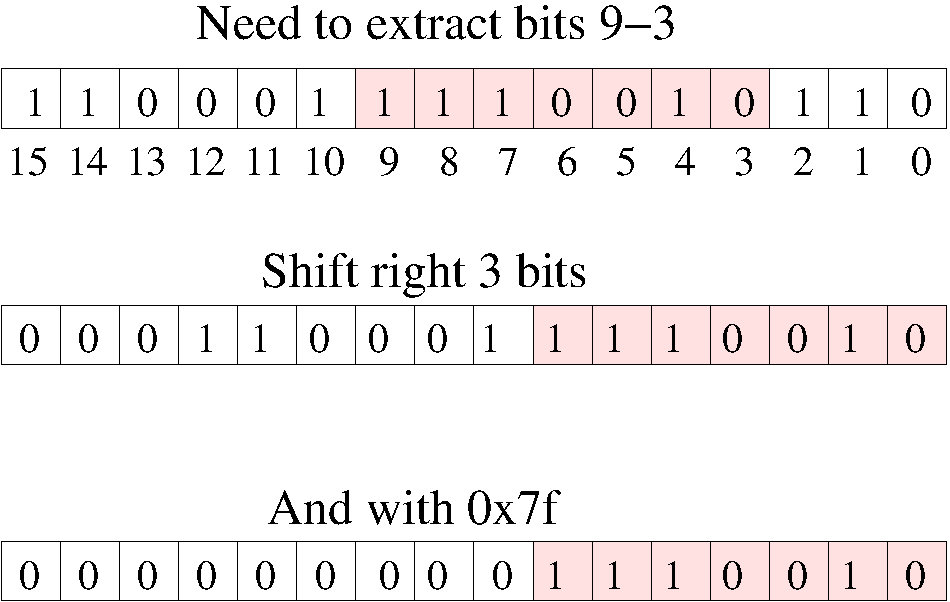
\includegraphics[width=4in]{extract_bits.pdf}
    \end{center}
\end{frame}

\begin{frame}
    \frametitle{Extracting a bit field with shift/shift}
    \begin{center}
        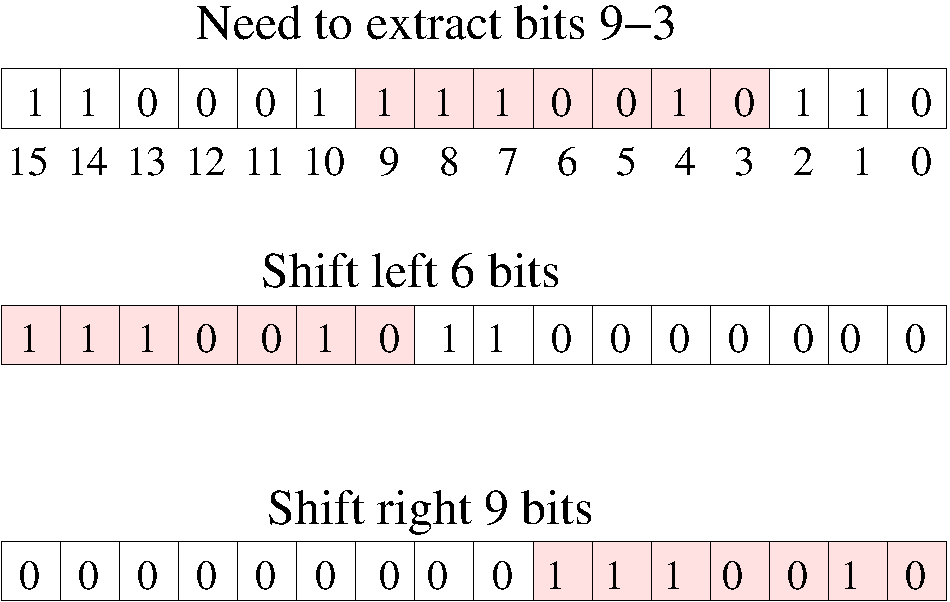
\includegraphics[width=4in]{extract_bits2.pdf}
    \end{center}
\end{frame}

\section{Rotate instructions}

\begin{frame}[fragile]
    \frametitle{Rotate instructions}
    \begin{itemize}
        \item The {\tt ror} instruction rotates the bits of a register
              or memory location to the right
        \item Values from the top end of the value start filling in the
              low order bits
        \item The {\tt rol} instruction rotates left
        \item Values from the low end start filling in the top bits
        \item These are 2 operand instructions like the shift
              instructions
        \item The first operand is the value to rotate
        \item The second operand is the number of bits to rotate
        \item The second operand is either an immediate value or {\tt
              cl}
        \item Assuming 16 bit rotates
    \end{itemize}
    \begin{verbatim}
    1 ror 2 = 0100000000000000b
    0xabcd rol 4 = 0xbcda
    0x4321 ror 4 = 0x1342
    \end{verbatim}

\end{frame}

\begin{frame}
    \frametitle{Filling a field}
    \begin{itemize}
        \item There are at least 2 ways of filling in a field
        \item You can shift the field and a mask and then use them
        \begin{itemize}
            \item Working with a 64 bit register, filling bits $m-k$
            \item Prepare a mask of $m-k+1$ bits all 1
            \item Shift the new value and the mask left $k$ bits
            \item Negate the mask
            \item And the old value and the mask
            \item On in the new value for the field
        \end{itemize}
        \item Use rotate and shift instructions and or in new value
        \begin{itemize}
            \item Rotate the register right $k$ bits
            \item Shift the register right $m-k+1$ bits
            \item Rotate the register left $m-k+1$ bits
            \item Or in the new value
            \item Rotate the register left $k$ bits
        \end{itemize}
    \end{itemize}
\end{frame}

\section{Bit testing and setting}

\begin{frame}[fragile]
    \frametitle{Bit testing and setting}
    \begin{itemize}
        \item It takes a few instructions to extract or set bit fields
        \item The same technique could be used to test or set single
              bits
        \item It can be more efficient to use special instructions
              operating on a single bit     
        \item The {\tt bt} instruction tests a bit
        \item {\tt bts} tests a bit and sets it
        \item {\tt btr} tests a bit and resets it (sets to 0)
        \item These are all 2 operand instructions
        \item The first operand is a register or memory location
        \item The second is the bit to work on, either an immediate
              value or a register
    \end{itemize}
\end{frame}

\begin{frame}[fragile]
    \frametitle{Set operations example code}
    \begin{itemize}
        \item {\tt rax} contains the bit number to work on
        \item This bit number could exceed 64
        \item We compute the quad-word of {\tt data} which 
              holds the bit
        \item We also compute the bit number within the quad-word
    \end{itemize}

\begin{verbatim}
    mov  rbx, rax           ; copy bit number to rbx
    shr  rbx, 6             ; qword index of data to test
    mov  rcx, rax           ; copy bit number to rcx
    and  rcx, 0x3f          ; extract rightmost 6 bits
    xor  edx, edx           ; set rdx to 0
    bt   [data+8*rbx],rcx   ; test bit
    setc dl                 ; edx equals the tested bit
    bts  [data+8*rbx],rcx   ; set the bit, insert into set
    btr  [data+8*rbx],rcx   ; clear the bit, remove
\end{verbatim}
\end{frame}

\end{document}
